\tikzset{
  basic/.style  = {draw, text width=2cm, rectangle},
  root/.style   = {basic, rounded corners=2pt, thin, align=center, fill=gray!30},
  level 2/.style = {basic, rounded corners=6pt, thin, align=center, text width=8em},
  level 3/.style = {basic, dashed, align=left, text width=6.5em, fill=gray!30}
}

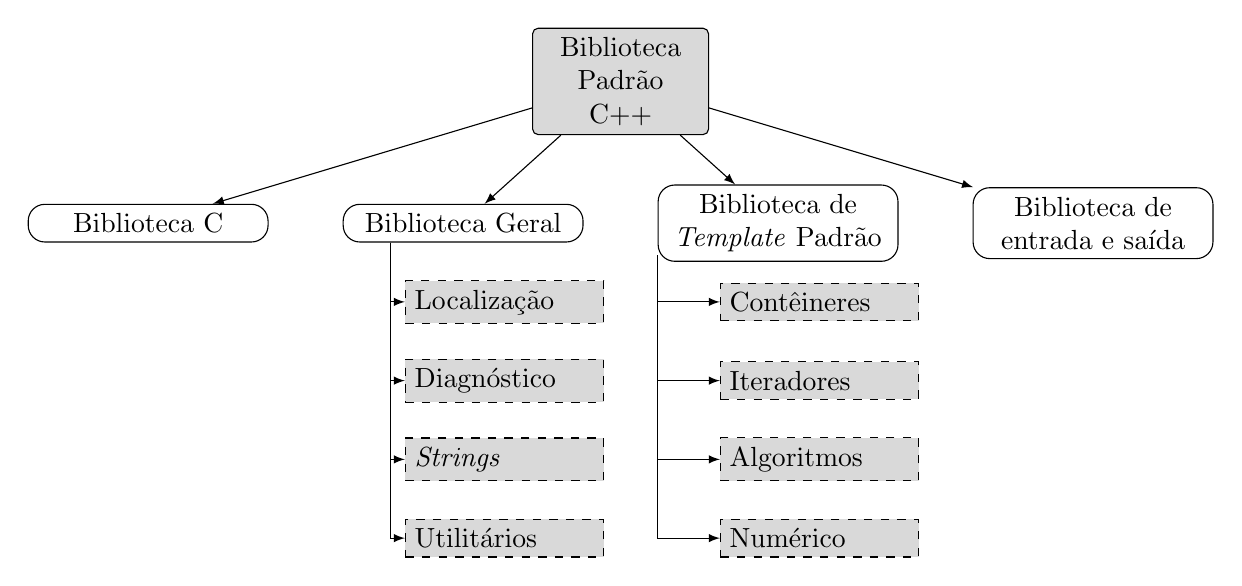
\begin{tikzpicture}[
  level 1/.style={sibling distance=40mm},
  edge from parent/.style={->,draw},
  >=latex, level distance=1.8cm]

% root of the the initial tree, level 1
\node[root] {Biblioteca Padr\~ao C++}
% The first level, as children of the initial tree
  child {node[level 2] (c1) {Biblioteca C}}
  child {node[level 2] (c2) {Biblioteca Geral}}
  child {node[level 2] (c3) {Biblioteca de \textit{Template} Padr\~ao}}
  child {node[level 2] (c4) {Biblioteca de entrada e sa\'ida}};

% The second level, relatively positioned nodes
\begin{scope}[every node/.style={level 3}]

\node [below of = c2, xshift=15pt] (c21) {Localiza\c c\~ao};
\node [below of = c21] (c22) {Diagn\'ostico};
\node [below of = c22] (c23) {\textit{Strings}};
\node [below of = c23] (c24) {Utilit\'arios};

\node [below of = c3, xshift=15pt] (c31) {Cont\^eineres};
\node [below of = c31] (c32) {Iteradores};
\node [below of = c32] (c33) {Algoritmos};
\node [below of = c33] (c34) {Num\'erico};
\end{scope}

\foreach \value in {1,...,4}
  \draw[->] (c2.195) |- (c2\value.west);

\foreach \value in {1,...,4}
  \draw[->] (c3.195) |- (c3\value.west);
\end{tikzpicture}